\subsection{Fouriersynthese}
\begin{figure}[h!]
	\centering
	\captionof{table}{Fourier-Koeffizienten}
	\begin{tabular}{c|ccc}
		& Dreieck & Rechteck & Sägezahn \\
		\hline
		k=1 & 628.84    & 631.02  & -627.10  \\
		k=2 & 0    & 0  & -313.60  \\
		k= 3 & 69.87  & 210.34  & -209.03  \\
		k= 4 & 0  & 0  & -156.78  \\
		k=5 & 25.15  & 126.20  & -125.42   \\
		k= 6 & 0  & 0  & -104.52  \\
		k = 7 & 12.83  &  90.1454 &  -89.59  \\
		k = 8 & 0 &  0 &  -78.39 \\
		k = 9 & 7.76 &  70.11 &  -69.68 \\
	\end{tabular}
	\label{tab:Koeffizienten}
\end{figure}
Die Fourierkoeffizienten $a_k$ werden für die Signale ausgerechnet.
\begin{align}
&\text{Dreieck:} \quad  a_k = \frac{8u}{(\pi k)^2}  \quad , k \in 2n + 1, n \in Z  \\
&\text{Rechteck:} \quad  a_k = \frac{4u}{k \pi} \quad , k \in 2n + 1, n \in Z \\
&\text{Sägezahn:} \quad a_k = - \frac{Tu}{kn \pi}
\end{align}
Wobei die Amplitude $u$ und die Periode $T$ der Funktionen konstant sind. Die ausgerechneten Koeffizienten stehen in Tabelle \ref{tab:Koeffizienten} und die Abbildungen der daraus generierten Signalverläufe \ref{Synthese_Dreieck}, \ref{Synthese_Rechteck}, \ref{Synthese_Saege} folgen darauf.



\begin{figure}[h!]
	\centering
	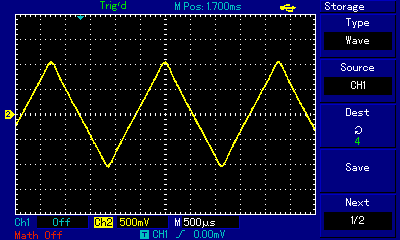
\includegraphics[width=0.9\textwidth]{Synthese_Dreieck.png}
	\caption{Annäherung an ein Dreiecksignal}
	\label{Synthese_Dreieck}
\end{figure}


\begin{figure}[h!]
	\centering
	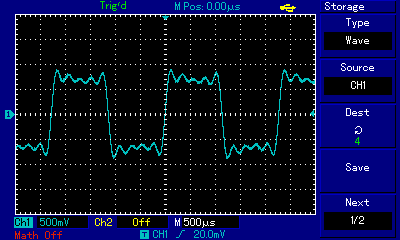
\includegraphics[width=0.9\textwidth]{Synthese_Rechteck.png}
	\caption{Annäherung an ein Rechtecksignal}
	\label{Synthese_Rechteck}
\end{figure}


\begin{figure}[h!]
	\centering
	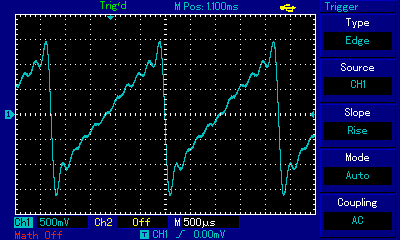
\includegraphics[width=0.9\textwidth]{Synthese_Saegezahn.png}
	\caption{Annäherung an ein Sägezahnsignal}
	\label{Synthese_Saege}
\end{figure}






\clearpage
\subsection{Fourieranalyse}
Für die Auswertung des Dreieck-, Rechteck-, und Sägezahnsignals werden die Fourierkoeffizienten eines eingespeisten Signals analysiert. In Unterkapiteln für jedes einzelne Signal befinden sich die Abbildungen, die am Oszilloskop zu sehen sind (Abbildung \ref{Frequenz_Dreieck}, \ref{Frequenz_Rechteck}, \ref{Frequenz_Saege}), Tabellen mit den abgelesenen und ausgerechneten Fourierkoeffizienten (Tabelle: \ref{tab:Dreieck}, \ref{tab:Rechteck}, \ref{tab:Saege})  und eine Visualisierung selbiger (Abbildung: \ref{Fourier_Dreieck}, \ref{Fourier_Rechteck}, \ref{Fourier_Saege}).
Die prozentuale Abweichung $\delta a$ der einzelnen gemessenen Koeffizienten $a_\text{gem.}$ von den errechneten $a_\text{ber.}$ ergibt sich nach
\begin{equation}
\delta a = \left(1 - \frac{a_\text{gem.}}{a_\text{ber.}}\right) \cdot 100 \%
\end{equation}
Die eingezeichneten Fehlerbalken beziehen sich auf die Gesamtabweichung von der erwarteten Funktion. Mehr dazu folgt in der Diskussion (Kapitel  \ref{sec:Diskussion}).
Sie wurden hier wie folgt berechnet
\begin{equation}
\Delta a =\sqrt{ \frac{1}{N-2} \sum_{i=2}^{N} (a_\text{gem.} - a_\text{ber.})^2 } \ .
\label{eq:Abweichung}
\end{equation}
Es ist wichtig, bei dem zweiten Wert zu beginnen, da der erste keine Abweichung haben kann. Deswegen wir auch durch $N-2$ geteilt, statt durch $N-1$.
\clearpage

\subsubsection{Dreiecksignal}

\begin{figure}[h!]
%	\centering
%	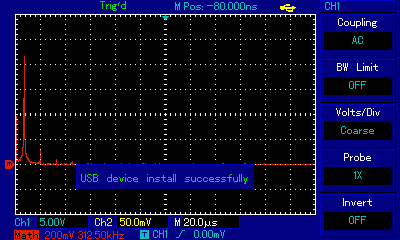
\includegraphics[width=0.6\textwidth]{Dreieck.png}
	\caption{Frequenzspektrum Dreiecksignal}
	\label{Frequenz_Dreieck}
\end{figure}

\begin{figure}[h!]
	\centering
	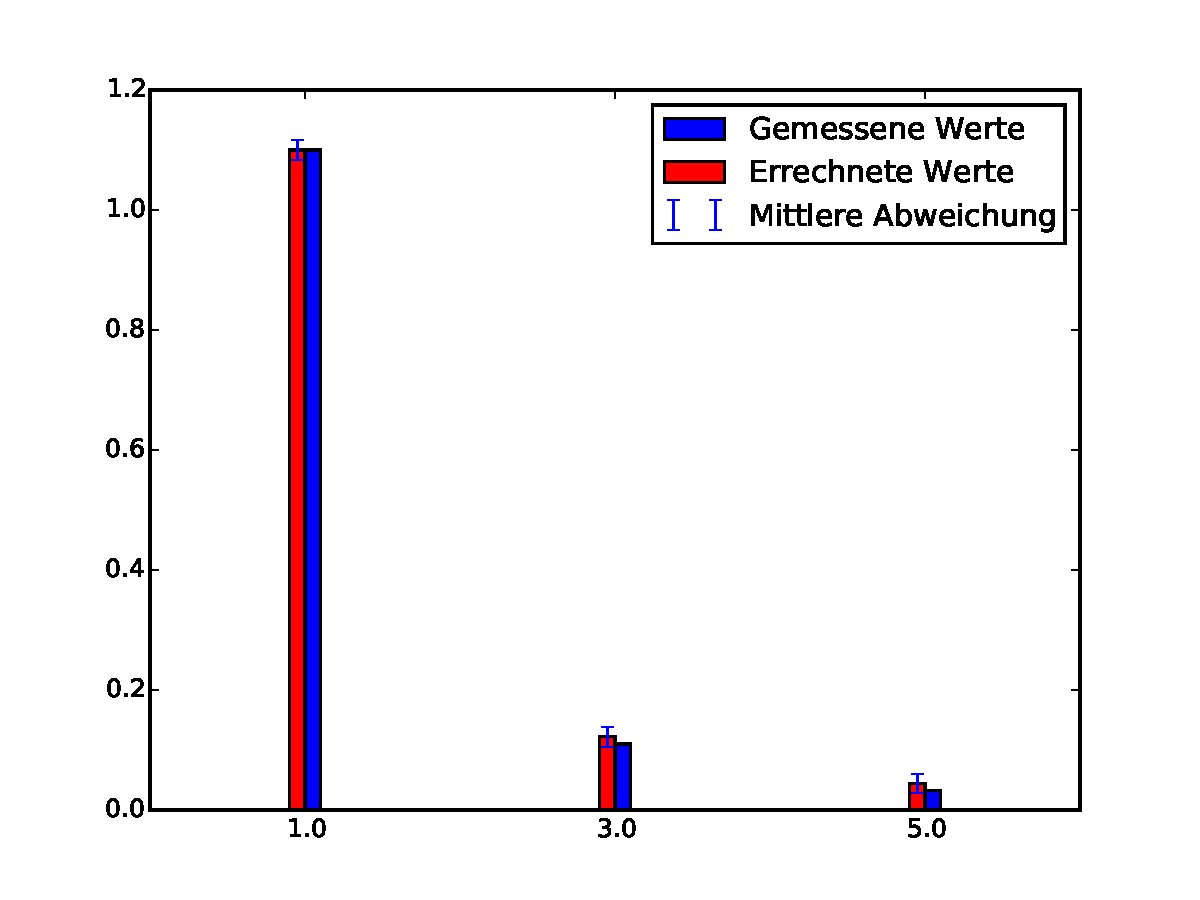
\includegraphics[width=0.6\textwidth]{Dreieck_Fourier.pdf}
	\caption{Frequenzspektrum Dreiecksignal}
	\label{Fourier_Dreieck}
\end{figure}

\begin{figure}[h!]
	\centering
	\captionof{table}{Fourier-Koeffizienten}
	\begin{tabular}{c|ccr}
		& gemessen in V & berechnet in V & Abweichung \\
		\hline
		k =	1 & 1.100   & 1.100      &  0 \%       \\
		k =	3 & 0.110  & 0.122 & -11 \% \\
		k =	5 & 0.033 & 0.044    & -33 \% \\
	\end{tabular}
	\label{tab:Dreieck}
\end{figure}
\clearpage



\subsubsection{Rechtecksignal}


\begin{figure}[h!]
	\centering
	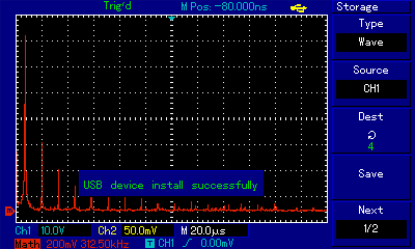
\includegraphics[width=0.6\textwidth]{Rechteck.png}
	\caption{Frequenzspektrum Rechtecksignal}
	\label{Frequenz_Rechteck}
\end{figure}

\begin{figure}[h!]
	\centering
	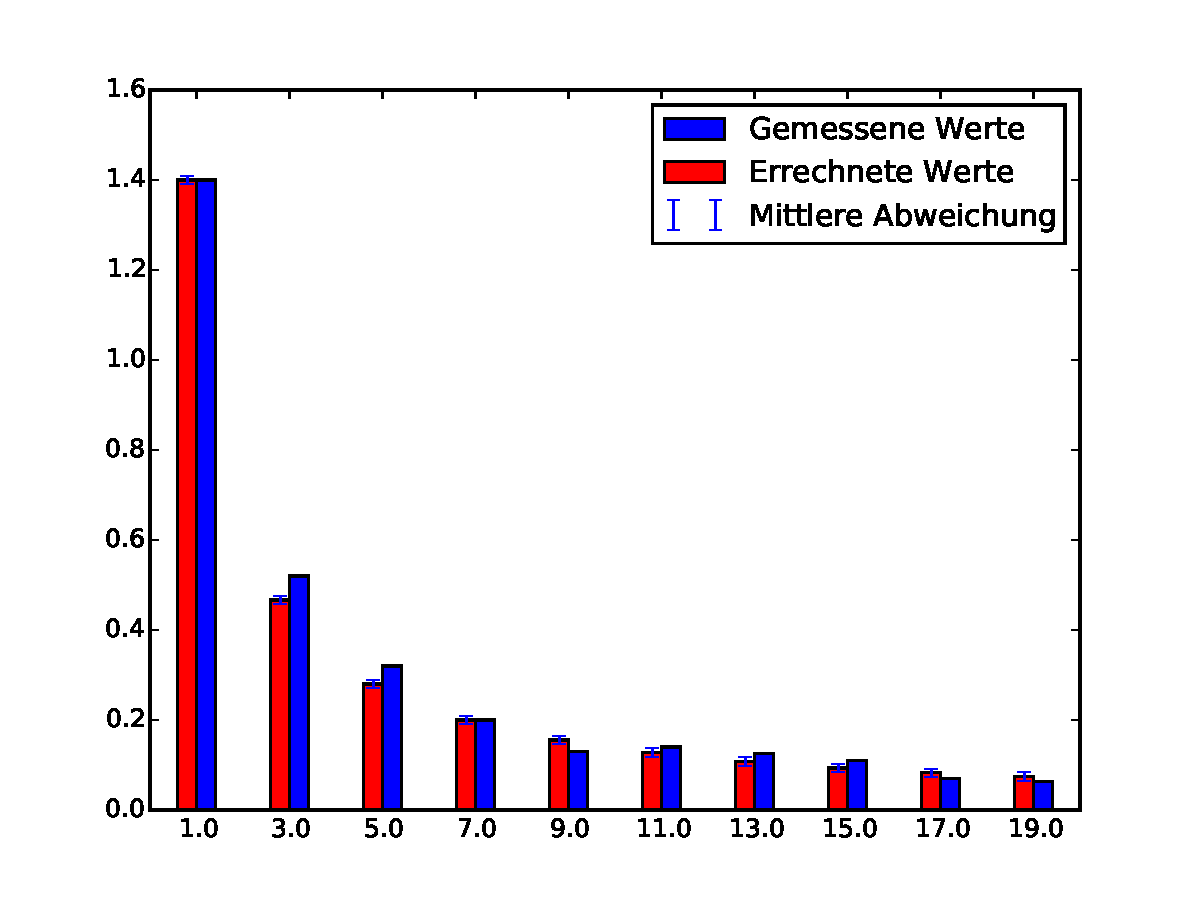
\includegraphics[width=0.6\textwidth]{Rechteck_Fourier.pdf}
	\caption{Frequenzspektrum Rechtecksignal}
	\label{Fourier_Rechteck}
\end{figure}

\begin{figure}[h!]
	\centering
	\captionof{table}{Fourier-Koeffizienten}
	\begin{tabular}{c|ccr}
		& gemessen in V & berechnet in V & Abweichung \\
		\hline
		k = 1 & 1.400   & 1.400       &  0   \%      \\
		k = 3 & 0.520  & 0.467 &  10.3 \%  \\
		k = 5 & 0.320  & 0.280      &  12.5  \%    \\
		k = 7 & 0.200   & 0.200       &  0  \%        \\
		k = 9 & 0.130  & 0.156  & -19.7 \%  \\
		k = 11 & 0.140  & 0.127  &  9.10 \% \\
		k = 13 & 0.125 & 0.108  &  13.8 \%  \\
		k = 15 & 0.110  & 0.093 &  15.2 \% \\
		k = 17 & 0.070  & 0.082 & -17.6 \%  \\
		k = 19 & 0.063 & 0.074 & -17.0 \% \\
	\end{tabular}
	\label{tab:Rechteck}
\end{figure}




\subsubsection{Sägezahnsignal}
\begin{figure}[h!]
	\centering
	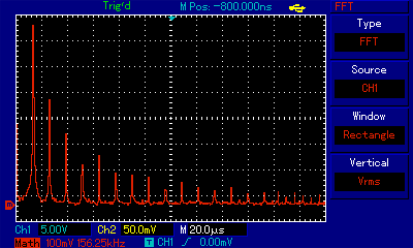
\includegraphics[width=0.6\textwidth]{Saegezahn.png}
	\caption{Frequenzspektrum Sägezahnsignal}
	\label{Frequenz_Saege}
\end{figure}

\begin{figure}[h!]
	\centering
	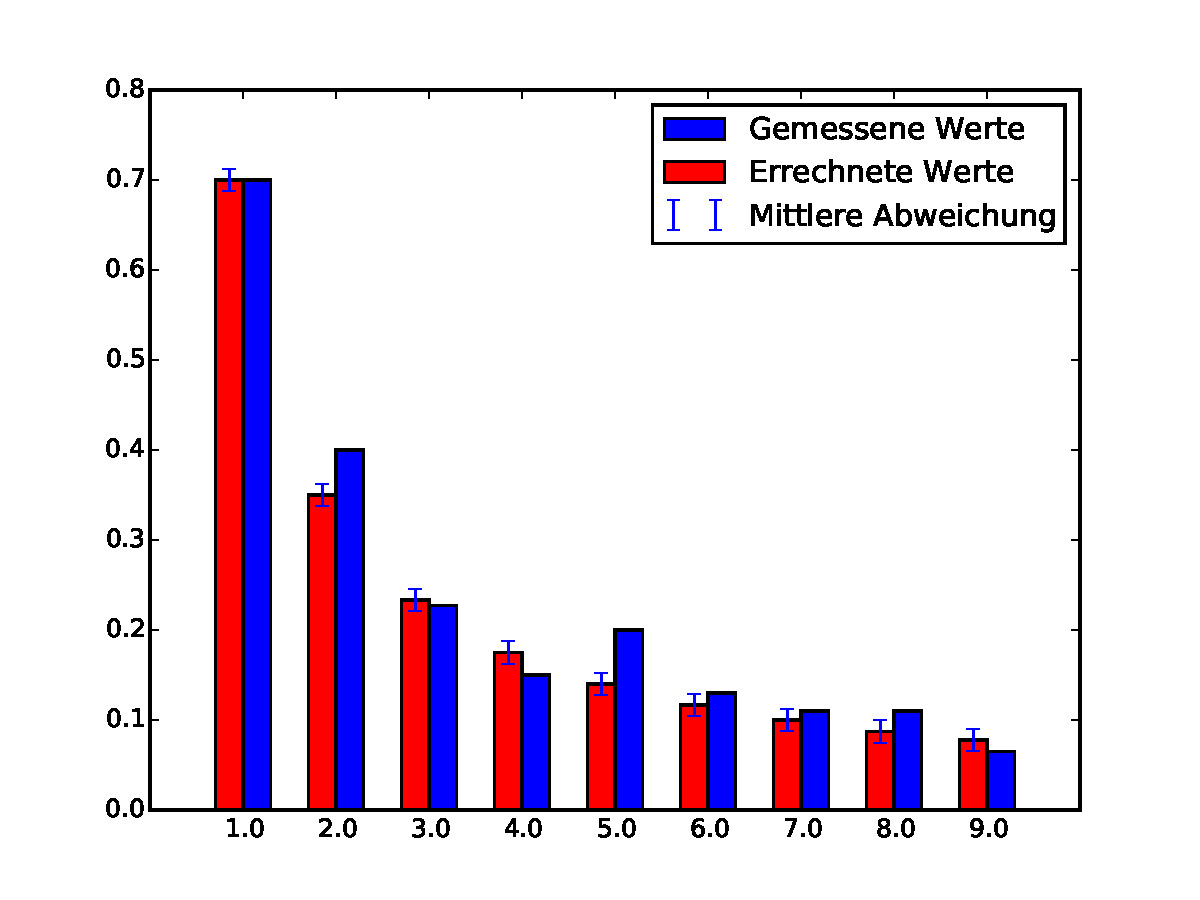
\includegraphics[width=0.6\textwidth]{Saegezahn_Fourier.pdf}
	\caption{Frequenzspektrum Sägezahnsignal}
	\label{Fourier_Saege}
\end{figure}

\begin{figure}[h!]
	\centering
	\captionof{table}{Fourier-Koeffizienten}
	\begin{tabular}{c|ccr}
		& gemessen in V & berechnet in V & Abweichung \\
		\hline
		 k = 1 & 0.700   & 0.700       &  0  \%       \\
		 k = 2 & 0.400   & 0.350      &  12.5 \%     \\
		 k = 3 & 0.227 & 0.233  & -02.8 \% \\
		 k = 4 & 0.150  & 0.175     & -16.7 \%  \\
		 k = 5 & 0.200   & 0.140      &  30.0 \%      \\
		 k = 6 & 0.130  & 0.117  &  10.3 \%  \\
		 k = 7 & 0.110  & 0.100       &  9.10 \% \\
		 k = 8 & 0.110  & 0.086    &  20.5 \%  \\
		 k = 9 & 0.065 & 0.078 & -19.7 \%  \\
	\end{tabular}
	\label{tab:Saege}
\end{figure}
\clearpage
